\documentclass[a4paper,10pt]{article}

%
%%% INPUT, FONTS, LAYOUT
%

\usepackage{fourier} % change this to change the font

\usepackage[english]{babel}   % Spacing and hyphenation rules for English.
\usepackage[T1]{fontenc} % ensures that ANSI characters <, >, | render correctly and are searchable

\usepackage[
  margin=15mm, 
  top=18ex,
  bottom=10ex, 
  footskip=5ex
]{geometry}


\usepackage{fancyhdr}
\pagestyle{fancy}
\fancyhead[L]{{\sffamily Feedlot working group}}
\fancyfoot[C]{}
\fancyfoot[R]{\thesection-\thepage}
\renewcommand \footrulewidth {2pt}

\usepackage{setspace} % provides \onehalfspacing, \doublespacing
\usepackage{calc} % provides length arithmetic
\usepackage{xcolor} % \color

\usepackage{graphicx}
\usepackage{verbatim}

  
\usepackage{amsthm}
\theoremstyle{remark}
\newtheorem*{example}{Example}

\newcommand{\defeq}{\mathrel{\vcenter{\hbox{\scriptsize:}}\!=}} % :=
\newcommand{\eqdef}{\mathrel{=\!\vcenter{\hbox{\scriptsize:}}}} % =:

%
%%% CROSS REFERENCING %%%%%%%%%%%%%%%%%%%%%%
%

\usepackage[colorlinks=true,
                linkcolor=teal,
                citecolor=olive,
                destlabel=true,
                bookmarks=true]{hyperref}

% Turns cross-references into links by redefining \refstepcounter
% Turns citations into links by redefining \bibcite
% Turns amsmath equation numbers into links by unknown wizardry
% Provides \href{}{}

\usepackage{bookmark} 
% patches hyperref to simplify processing (no .out file is generated and 
% only needs 2 runs).

%
%%% BIBLIOGRAPHY %%%%%%%%%%%%%%%%%%%%%%%%%%


\usepackage[style=authoryear]{biblatex}
\setcounter{biburllcpenalty}{1}   % freely break URLs at lowercase

% use \addbibresource to register .bib databases

\addbibresource{master.bib}

% About backends:
% bibtex reads both the .aux file and .bib file.
% biber reads ONLY the .bcf file which is generated by biblatex 
% when backend=biber.
%
% About biblatex:
% loads etoolbox
% Use \nopp to suppress p. pp. in postnote. 
% Alternatively, change pagination field in bib entry.
% For arXiv compatibility require versions:
%  .bbl format 2.8 biblatex 3.7 Biber 2.7
%  (as of May 2020, arXiv uses TeXLive 2016)

\usepackage{csquotes} % prevents a warning for using biblatex with babel



\DeclareBibliographyDriver{eprint}{%
  \usebibmacro{bibindex}%
  \usebibmacro{begentry}%
  \usebibmacro{author/editor+others/translator+others}%
  \setunit{\printdelim{nametitledelim}}\newblock
  \usebibmacro{title}%
  \newunit
  \printlist{language}%
  \newunit\newblock
  \usebibmacro{byauthor}%
  \newunit\newblock
  \usebibmacro{byeditor+others}%
  \newunit\newblock
  \printfield{howpublished}%
  \newunit\newblock
  \printfield{type}%
  \newunit
  \printfield{version}%
  \newunit
  \printfield{note}%
  \newunit\newblock
  \usebibmacro{organization+location+date}%
  \newunit\newblock
  \usebibmacro{eprint}%
  \newunit\newblock
  \usebibmacro{addendum+pubstate}%
  \setunit{\bibpagerefpunct}\newblock
  \usebibmacro{pageref}%
  \newunit\newblock
  \iftoggle{bbx:related}
    {\usebibmacro{related:init}%
     \usebibmacro{related}}
    {}%
  \usebibmacro{finentry}}


%%% MATH MACROS %%%%%%%%%%%%%%%%%%%%%%%%%%%%%

\newcommand \Vol {\mathrm{vol}}
\newcommand \oracle {\mathcal{O}}


%
%%% TITLE & SPLASH
%

\usepackage{titling}

\pretitle{
  \begin{flushleft} \Huge \sffamily \rule{\textwidth}{0.1ex}\vspace{1ex}}
\posttitle{ \rule{\textwidth}{0.1ex} \end{flushleft}}
\title{ Feedlot: trading with safe, low latency price oracles  \thanks{This research was funded by the Gnosis DAO.} }

\preauthor{\begin{flushleft} \LARGE \sffamily \itshape}
\author{The Feedlot working group}
\postauthor{\end{flushleft}}

\date{}


\newcommand \printsplash {%
\noindent
  { \color {gray} \rule[-1ex]{0.5em}{7ex}\hspace{2em} }
  \begin{minipage}[b]{\textwidth - 4.7em}
    \onehalfspacing
    \emph{feed} --- Something supplied continuously.
    
    \emph{lot} --- One or more items auctioned or sold as a unit, separate from other items.
  \end{minipage}
  { \color {gray} \rule[-1ex]{0.2em}{7ex}\hspace{2em} }
  \vspace{4ex}
}

%%% END OF PREAMBLE %%%%%%%%%%%%%%%%%%%%%%%%%

\begin{document}
\maketitle
\printsplash

\paragraph{Abstract}

This article is a feasibility study for a class of automated market makers (AMMs), collectively dubbed \emph{Feedlot}, that passively provide liquidity at a price based on the uniform clearing price (UCP) of a competitive batch auction such as CoW protocol.
%
If appropriately implemented, liquidity providers on Feedlot AMMs should enjoy protection from the adverse selection that plagues CFMM LPs, and oracle fees could provide a new revenue stream for the batch auction provider itself.

We review general principles of designing CFMMs and pricing oracles; propose an architecture for a channel through which the CoW UCP is communicated to a liquidity pool; and review the security implications for CoW and trading through the UCP liqudity pool. From theoretical and empirical perspectives, we study the economic implications for traders and LPs that a functioning Feedlot implementation would entail.

This article is not a whitepaper, specification, or fully fleshed out proposal, and it makes no claim to exhaustiveness or completeness on any of the topics discussed --- particularly security. 
%
Would-be implementers of a Feedlot AMM are advised to pursue thorough further investigations of these issues in the context into which they hope to deploy.

\section{Introduction}

The most widely used type of blockchain market today is the constant function automated market maker (CFMM), whose deployments collectively process trading volume to the value of tens of billions USD per month \cite{buterin2016lets, adams2020uniswap, oneill2023can}.
%
A CFMM provides an environment where anyone can deploy funds and passively accept trades in exchange for trading fees.
%
Price impact is calculated in terms of the reserves using highly space and time efficient algorithms.

The popularity of the CFMM model has brought to light some basic difficulties.
%
In addition to fundamental risk, liquidity providers on CFMMs are exposed to the effects of \textbf{adverse selection}: they incur losses from being forced to accept trades with informed actors at unfavourable prices.  
%
Many groups of liquidity providers consistently lose money on their investment \cite{loesch2021impermanent}.
%
Meanwhile, the permissionless and public environment in which CFMMs execute exposes na\"ive traders to the activities of MEV bots, who take advantage of the trader's revealed intentions together with the market's deterministic price impact function to manipulate prices and extract value from a pending transaction \cite{zhou2021high, holloway2023value}.

Various schemes have been proposed to address some of the issues associated with fully automated markets \cite{ferreira2022credible, josojo2022mev, nikete2022towards, fleupold2022cow}.
%
Some aim to protect users by providing a dedicated channel that provides additional privacy, failure, or ordering guarantees.
%
Among these, blockchain implementations of the \emph{RFQ batch auction model} socialise pricing and protection from ordering attacks by settling trades atomically in batches with a \emph{uniform clearing price} (UCP).
%
This price is provided by the winner of a competition to find routes for orders that maximise the welfare of their creators.

Another class of proposals adopts the idea of adjusting pricing using an external price feed \cite{dodoex,synthetixlitepaper}.
%
If this price feed is sufficiently reliable, passive liquidity providers can mitigate or even entirely avoid losses to adverse selection.
%
However, employing such a price feed for trading provides a strong incentive to deliberately skew, interrupt, or otherwise manipulate the published price.
%
A typical price feed pipeline has several phases that could fail --- by accident or design --- to preserve the integrity of the published data. 
%
Examples of cases where financial losses have occurred as a result of relying on such feeds are plentiful \cite{liu2021first, cryptocat2020how, venus2022luna, eskandari2021sok}.

This report discusses a proposal to use the UCP provided by an RFQ batch auction with on-chain settlement --- specifically, CoW protocol\footnote{\url{https://docs.cow.fi}} --- to adjust the pricing of a liquidity pool.
%
The fact that the UCP is used to settle a batch auction means that it has a unique guarantee not shared by other price oracle data sources: it is \emph{realisable} in the sense that it comes with an on-chain proof that it could be used to execute trades (at least, before the batch).\footnote{In the language of \cite{suresh2022so}, it is backed by \emph{trade collateral}.}

Based on this model, we give the working name \emph{Feedlot} to a hypothetical AMM.
%

The rest of this report is structured as follows: in \S\ref{general}, we review general principles of designing CFMMs and pricing oracles; 
%
in \S\ref{architecture} we discuss the channel through which the UCP is communicated to a Feedlot liquidity pool; 
%
in \S\ref{security} we review the security implications for CoW and Feedlot of consuming the UCP to execute additional trades;
%
finally, in \S\ref{impact} we study the economic implications for traders and LPs that a functioning Feedlot implementation would entail from theoretical and empirical perspectives.


\section{General design principles}
\label{general}

\subsection{Definitions}

Our blockchain model is based on Ethereum, and should apply to any blockchain-based state machine with similar principles (for example Gnosis Chain).
%
\begin{comment}
In particular we point out the following assumptions:
\begin{itemize}
\item Accounts model that tracks token balances with a common interface (e.g. ERC20) and such that token transfers satisfy usual invariants (i.e.~transfers must preserve total supply and balances cannot be negative).
\item Transactions (a.k.a.~messages calls) must be initiated by an off-chain entity.
\item Transactions, once committed, cannot be rolled back. That is, we do not consider the risk of blockchain forks.
\end{itemize}
\end{comment}
By a \emph{smart contract system} we mean any kind of on-chain entity or aggregation of entities. In particular, it may mean a single smart contract (e.g.~a Uniswap pool) or a structured collection of interacting smart contracts (e.g.~Uniswap as a whole).

We make use of the following standard terminology:
\begin{itemize}

  \item \emph{Liquidity pool.} Smart contract system that custodies the assets of \emph{liquidity providers} and tracks withdrawal liabilities.
  
  \item \emph{Liquidity provider (LP).} An agent that deposits funds in a liquidity pool.
  
  \item \emph{Automated market maker (AMM).} Smart contract system that provides pricing and passively settles orders by trading against a liquidity pool.
  
  \item \emph{Batch auction.} Order settlement system that accumulates orders in a buffer and settles them with a uniform clearing price.
  %
  Prices are supplied by \emph{solvers} who compete to optimise an objective function defined in terms of the price vector and the set of orders.
  
  \item \emph{Uniform clearing price (UCP).} Price vector against which a batch auction is settled.
  
  \item \emph{Coincidence of wants (COW).} Execution or partial execution against one another of two orders in opposing directions. 
  
  \item \emph{Solver.} Agent that provides quotes in competition to settle a batch auction.
  
  \item \emph{Constant function market maker.} An AMM whose pricing function depends only on reserves.
  
\end{itemize}

For simplicity, we will consider only liquidity pools with two assets $A$ and $B$ whose balances are denoted $(x,y)\in [0,\infty)^2$.
%
We take token $A$ for the num\'eraire (also called the `quote token'), so that prices are for token $B$ in terms of token $A$.
%
If a trade occurs of $\Delta x$ $A$ tokens for $\Delta y$ $B$ tokens, the execution price is $\Delta x/\Delta y$.

\subsection{Constant function market makers}

A constant function market maker (CFMM) is defined by its \emph{invariant function} $f(x,y)$, a real-valued function of the pool reserves.
%
The associated marginal pricing function is 
\[
  p(x,y) = \frac{f_x(x,y)}{f_y(x,y)}.
\]
If reserves are in state $(x_0,y_0)$, the amount of $B$ tokens paid out in exchange for $-\Delta x$ $A$ tokens is
\[
  \Delta y = \int_{x_0}^{\Delta x} 1/p(x,y(x))dx - y_0
\]
where $y(x)$ is determined by the corresponding differential equation $y'(x) = 1/p(x,y(x))$ and the initial conditions $y(x_0)=y_0$.

A practical implementation of market orders on a CFMM must have a computationally efficient algorithm for computing $\Delta y$ given $\Delta x$.
%
On the other hand, to decide if a given swap $(\Delta x, \Delta y)$ will be accepted by a CFMM, it is enough to compute the invariant $f(x+\Delta x,y+\Delta y)$.

\subsection{Liquidity provider costs}

The CFMM quote is not automatically updated when changes occur on other markets. 
%
Rather, price updates are supplied by arbitrageurs who trade on the CFMM in such a way as to push the pricing into alignment with external markets. 

From a dual perspective, this trading activity has the effect of adjusting the balance of assets in the pool towards the value-minimising point on the level curve, computed in terms of external market prices. 
%
For example, with Uniswap's constant product formula $f(x,y)=xy$, the equilibrium balance is 50-50, that is, $px=y$.

LPs effectively pay for this adjustment service by trading at unfavourable prices \cite{milionis2022automated}.
%
The amount they pay depends only on the external price movement and the second derivative of the optimal pool value function.
%
In particular, there is no room for price updaters to compete with one another on the basis of reducing cost to LPs; rather, all arbitrageur competition is at the infrastructure layer and excess rewards tend to be absorbed either by consensus nodes or by middleware services that assemble blocks or partial blocks \cite{daian2020flash}.
%
LPs cannot concentrate liquidity near a single price without exposing themselves to more severe adverse selection impact.

\subsection{Automated market makers with a price feed}
\label{price-feed}

The issue of uncontrolled LP losses to adverse selection could be alleviated if price updates from external markets could be supplied by another channel, so that the marginal pricing function could depend on inputs other than reserves:
\[
  p = p(x,y;p_\mathrm{ext}).
\]
%
In blockchain applications, such channels are called \emph{price oracles} \cite{heiss2019oracles, muhlberger2020foundational, albreiki2020trustworthy}.

\begin{example} The most obvious choice for an oracle-based pricing function is
\[
  p(x,y;p_\mathrm{ext}) = p_\mathrm{ext},
\]
so that the AMM simply quotes the oracle price.
%
We refer to this as \emph{passthrough} pricing.
%
If we black-box the data source and assume that it provides no-arbitrage prices, then such an AMM would indeed be protected from adverse selection. \end{example}

However, as is well-known, oracles in the field are fallible.
%
They are vulnerable to bugs and deliberate attacks at each stage of the data pipeline.
%
Oracles that provide prices that anyone can trade against are a particularly attractive vector for sabotage, both because of the potential for financial gain and because, in the case of a manipulated data source, of the difficulty in establishing that an attack has even occurred \cite{samczsun2020so, suresh2022so}.

Moreover, simply passing through the oracle price offers no control over inventory management.
%
In particular, if trading tends to occur more on one side than the other for whatever reason, reserves of the in-demand asset could easily dry out \cite[\S2.2]{garman1976market}.
%
In traditional finance, this risk is typically accounted for by adjusting pricing to be more or less favourable depending on whether a trade would push reserves towards or away from the desired inventory \cite{biais2005market}.
%
Assuming a typical microeconomic environment with negatively sloped demand curves, order flow naturally skews towards the buy (resp.~sell) side as prices edge below (resp.~above) the market clearing price.
%
If prices slide far enough for arbitrages to appear, one can further suppose that a population of informed traders will rapidly effect the desired inventory adjustments.

\begin{example}
  Suppose we target a reserve balance of 50-50 (computed in terms of the oracle price), setting
  \[
    p(x,y;p_\mathrm{ext}) = p_\mathrm{ext}\cdot g\left(x/yp_\mathrm{ext}\right)
  \]
  where $g:(0,\infty)\rightarrow(0,\infty)$ is a monotone increasing function such that $g(1) = 1$.
  %
  The most basic choice is $g(r)=r$, in which case the price oracle drops out of the formula and we recover the UniswapV2 pricing function $p(x,y;p_\mathrm{ext})=x/y$.
\end{example}

\begin{example}
  More interesting is to choose a function which has a small or vanishing gradient near $1$. A simple example is
  \[
    g(r) = \left\{\begin{array}{ll}
      r\kappa & r \leq \kappa^{-1} \\
      1           & \kappa^{-1} \leq t \leq \kappa \\
      r\kappa^{-1} & \kappa\leq r
    \end{array}\right.
  \]
  where $\kappa >1$ is the `tolerance ratio' of the pool for reserves to deviate from an even balance.
  %
  \begin{figure}
    \begin{center} 
      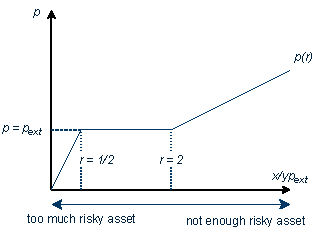
\includegraphics{diagrams/price-curve.pdf}
      \caption{Piecewise linear pricing function of reserve balance with tolerance ratio $\kappa = 2$.}
    \end{center}
  \end{figure}
  %
  An AMM trading on this pricing function provides passthrough pricing as long as the inventory balance remains in the range $[\kappa^{-1},\kappa]$; a simple calculation shows that outside that range it trades as a weighted CPMM with weights $(1,\kappa)$, resp.~$(\kappa,1)$, depending on whether we have too little num\'eraire or too much, respectively.
  
  More generally, `stableswap' curves used in the wild for liquidity pools with weakly pegged prices can be adapted using this price feed approach to trade volatile assets as well \cite{egorov2019stableswap, port2022mixing}.

\end{example}

\begin{example}

  Yet another approach is to provide CPMM pricing, but bound execution prices by the oracle price in the direction unfavourable to the LP.
  %
  This is similar to the pricing function approach in that the CPMM preference curve discourages trading that would push the inventory too far from the desired balance, but the normalisation of this curve updates only when the AMM accepts a trade, rather than when the oracle updates.
  %
  The hybrid model has the benefit of ease of implementation.
  
\end{example}

\subsection{Design goals}

A successful implementation of a Feedlot AMM should have the following properties:
\begin{itemize}
  \item
    Liquidity providers should enjoy cheap portfolio management, some yield, and protection from adverse selection.
    
  \item
    Traders should enjoy low, predictable fees, control over execution time, and favourable prices at least for trades in the `correct' direction.
    
  \item
    It should not be economical to manipulate the uniform clearing price (UCP) of the CoW batch auction in order to trade at favourable prices on Feedlot.
    
    Moreover, it should not be possible to substantially offset the cost of manipulating the CoW UCP (for any reason) by trading on a Feedlot AMM.

  \item 
    Wherever possible, Feedlot should use incentive-compatible mechanisms to ensure correct operation.
    %
    Social adjudication procedures should be employed only as a fallback.
  
\end{itemize}
%
In subsequent sections, we discuss approaches to implementing an AMM realising this list.


\section{Architecture}
\label{architecture}

Our model for a batch auction system is the CoW protocol on Ethereum.
%
The CoW protocol consists of a set of off-chain entities that we collectively refer to as \emph{CoW services} and a system of Ethereum smart contracts called the \emph{CoW contracts}. The details of the internal architecture of these aggregations is not discussed here.

Schematically, the CoW algorithm runs as follows:
\begin{enumerate}
  \item 
    Traders send orders to an off-chain order book server where they are tracked in a database.
    
  \item 
    A set of offchain entities called \emph{solvers} query the database and attempt to construct a \emph{solution}, that is, an Ethereum transaction that collectively settles all user orders at a fixed price vector $\vec{p}$ --- the uniform clearing price.
    %
    This transaction may contain arbitrary Ethereum message calls.
    
  \item
    Every batch interval, solutions are validated by simulating against a recently observed chain state and ranked according to a utility function.
    %
    The utility function measures the total marginal utility of user orders filled by the solution in terms of the difference between the limit price and the fill price.
    %
    Utilities of orders denominated in different tokens are normalised using prices on whitelisted external markets.
    
  \item
    The solver with the winning solution calls the \texttt{settle()} function on the CoW settlement contract, which executes their solution, emitting \texttt{Trade} events.
    
  \item
    Misbehaviour is assessed socially. Slashing punishments can be triggered by a vote of the CoW DAO.
\end{enumerate}
\begin{figure}
  \begin{center}
    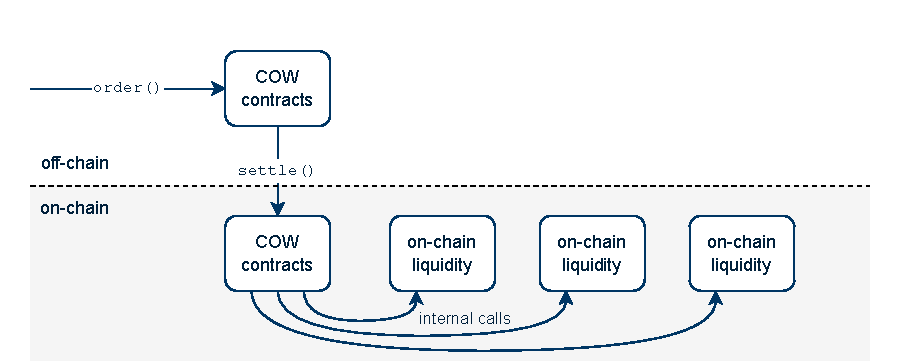
\includegraphics[width=\textwidth * \real{0.8}]{diagrams/cow2.pdf}
    \caption{CoW procotol execution. CoW services accumulate orders and batches are settled (at most) every 30 seconds.}
  \end{center}
\end{figure}
%
An AMM whose quote depends on the UCP of the CoW batch auction needs to have at least the following structures:
\begin{itemize}
  \item A way for traders to submit orders.
  \item A way for would-be LPs to add or remove liquidity.
  \item A communication channel $\mathcal{O}$ connecting Feedlot with the CoW contracts or services along which can be communicated the UCP.
\end{itemize}
The first two components are standard elements of AMM implementation. 
%
The last item is the distinguishing feature of Feedlot AMMs, so in this section we focus on the design of this channel.

\subsection{Synchronisation}

A batch auction system needn't be synchronised with the blockchain.
%
There may not be an auction every block, and even if there is, not every token pair traded on the BAS need necessarily appear in the batch.
%
This is the case for CoW: auctions are roughly every 30 seconds, and sometimes no auction occurs for hours at a time.
%
Therefore, a fresh batch auction price might not be available at the point that a trader wishes to trade on feedlot.

If the Feedlot quote price is to depend on the price of a CoW batch auction, then, there are only two possibilities:
\begin{enumerate}
  \item The quote function uses a stale CoW price (poll model).
  \item The market only settles trades at the same time as the batch auction (subscription model).
\end{enumerate}
These two options are analogous to what in the blockchain oracles literature have been called the \emph{pull} and \emph{push} models, respectively \cite{heiss2019oracles,muhlberger2020foundational}.

In either case, CoW services can guarantee zero latency updates of the UCP by writing into the channel atomically together with the batch execution transaction. 
%
This would require minor modifications to CoW's offchain components so that they call a wrapper contract that both triggers the CoW settlement and publishes a price to the on-chain oracle.
%
It does not require any changes to CoW's onchain components.
%
\begin{figure}
  \begin{center}
    \vspace{2ex}
    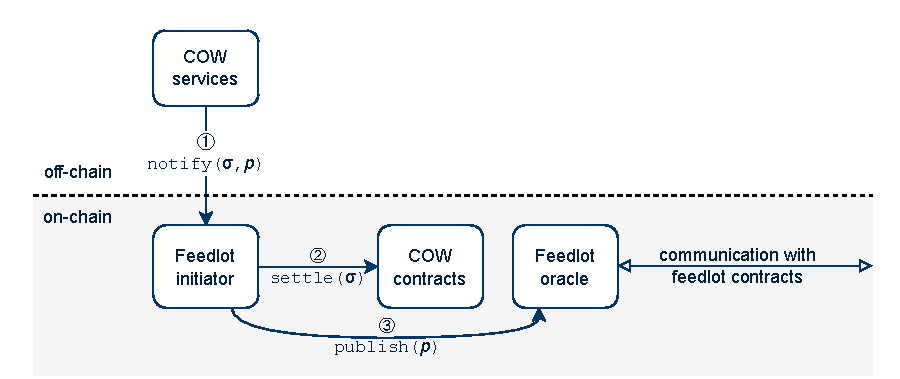
\includegraphics[width=\textwidth * \real{0.8}]{diagrams/wrapper.pdf}
    \caption{Atomic execution of the batch solution and publication of the UCP. The ordering of (2) and (3) can be reversed.}
  \end{center}
\end{figure}
%

What could be considered a third option is to fall back on another algorithm in case no price is available. 
%
Since that essentially amounts to not trading on Feedlot, and could easily be implemented at a higher layer, we don't discuss that here.

\subsubsection{Poll model}

In this model, CoW writes the UCP vector to the channel every time there is a batch. Meanwhile, Feedlot AMMs query the price whenever they have to settle an order.
%
There is no synchronisation between these two tasks.
%
One write is needed per batch per product, and one read is needed per trade on Feedlot.
%
These operations being relatively cheap, it would be reasonable to implement this type of channel as an on-chain oracle.
%
\begin{comment}
\begin{figure}
  \begin{center}
    \vspace{1ex}
    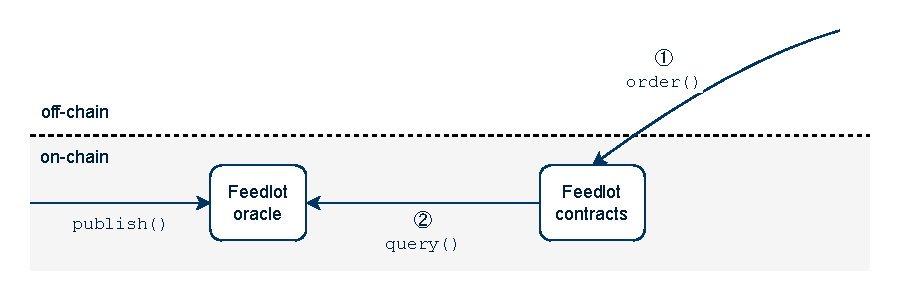
\includegraphics[width=\textwidth * \real{0.8}]{diagrams/poll.pdf}
    \caption{Polling oracle. Feedlot AMM executions are not synchronised with CoW batches.}
  \end{center}
\end{figure}
\end{comment}
%
A variant approach is to aggregate UCPs to produce, for example, time-weighted average prices. This is the approach taken by Uniswap's oracle service \cite{adams2020uniswap}.

Since the prices retrieved by this method are necessarily stale, this approach does not preserves the unique \emph{realisability} property of the UCP (see \S\ref{realisable}). For this reason, and because poll-based oracle services are already plentiful, for the rest of this report we focus instead on the more interesting subscription model.

\subsubsection{Subscription model}

In this approach, orders arriving at Feedlot are accumulated in an order book.
%
All trades are executed when there is a CoW batch.
\begin{comment}
\begin{figure}
  \begin{center}
    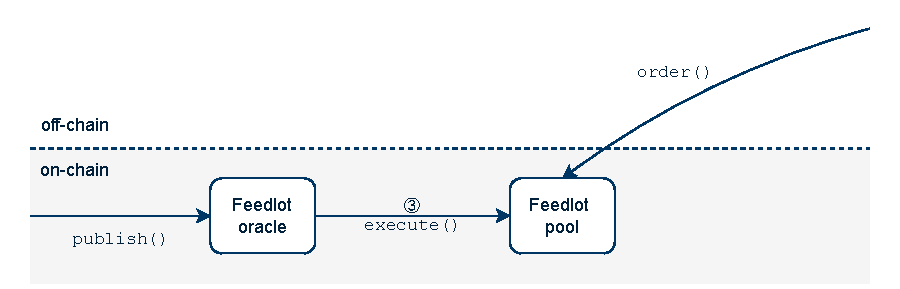
\includegraphics{diagrams/sub.pdf}
    \caption{Subscription oracle. Feedlot AMM executions are triggered when a new price is published.}
  \end{center}
\end{figure}
\end{comment}
%
Whether the Feedlot trades execute before or after the CoW batch affects only how Feedlot behaves for orders placed in the winning solution itself; see \S\ref{solution-on-feedlot}.
%
Orders that arrive at Feedlot outside the batch are not affected by this ordering.

As with any order book based protocol, the order book itself would potentially be quite expensive to maintain on the Ethereum chain.
%
It is beyond the scope of this report to discuss approaches for optimising trust model and cost-effectiveness of off-chain order books.
%
Pragmatically, a reasonable approach would be to maintain the order book in the same place as the order book for the CoW batch auction, which at time of writing is a set of servers maintained by the CoW team.
\begin{figure}
  \begin{center}
    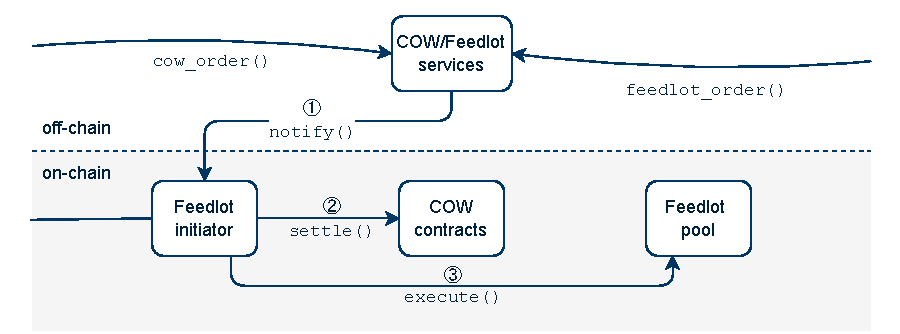
\includegraphics{diagrams/sub-merged.pdf}
    \caption{Integrated oracle with offchain order queue. Feedlot AMM executions are triggered when a new price is published.}
  \end{center}
\end{figure}

\subsection{Can the batch itself settle on Feedlot?}
\label{solution-on-feedlot}

Certain configurations would allow the solution itself to both settle orders on Feedlot and quote it a price.
%
Evidently, this can only happen if Feedlot orders are executed \emph{after} execution of the solution but \emph{before} verifying that the solution satisfied all the orders it claimed to satisfy.
%
We call this model \emph{CoW native}, because in this case only the CoW batch solution can interact directly with the AMM; here Feedlot acts as a kind of private liquidity pool for solvers.
%
Note also that in this case, AMM orders do not have to wait in a queue to be executed (though of course, the user orders being settled by the batch had to wait for the batch as usual).

Implemented na\"ively, this design permits the winning solver to quote any price at all and have it instantly execute against Feedlot.
%
Since the solver's objective is to get the most favourable price possible for its users, a rational solver will quote the least favourable price that Feedlot will accept.
%
Naturally, allowing an entity to trade against the AMM at any price it chooses is trivially exploitable to the detriment of LPs, and so special care has to be taken to address this case.
%
While the ability for solvers to both set prices and trade at those prices on Feedlot persists even when the batch  itself cannot settle on Feedlot --- see \S\ref{security} --- this design is the only situation in which doing so is completely risk-free for the solver.

Nonetheless, some of the mitigation strategies discussed in \S\ref{mitigation} still apply to this case.
%
By adjusting the solver objective function and by carefully defining and monitoring solver activities, it may be possible to make a CoW native AMM that protects its LPs from adverse selection while providing a safe execution environment for solvers.


\begin{comment}
Let us discuss, and dismiss, in turn a few approaches to making this work:
\begin{itemize}
  \item 
    Bound Feedlot's pricing function below independently of the UCP. For example, accept a trade only if it offers better pricing for the pool than some hardcoded aggregate of prices from whitelisted external markets.
    %
    Then rational solvers will always trade at exactly this lower bound.
    %
    This eliminates the dependence of pricing on the UCP.
    
  \item
    Adjust the solution objective to some strictly convex function that takes into account utility of the pool as well as active traders.\footnote{If it isn't \emph{strictly} convex, solvers will be indifferent between delivering utility to traders or the pool.}
    %
    The objective function will have to be normalised so that, independently of absolute price, it achieves some desired balance between pool and trader utility.
    %
    Clearly, this price normalisation cannot be derived from the price quoted by solvers, because as before they would then be free to set it arbitrarily.
    %
    Hence, an auxiliary price oracle is needed.
    
  \item
    Allow solutions that successfully simulate on markets other than Feedlot to actually settle instead on Feedlot, at the price that was realisable on those markets.
    %
    This has the effect of making price manipulation costless: solvers can provide their own liquidity at any price, knowing that they will not be held to trading at that price, this burden ultimately falling on Feedlot LPs.
    
\end{itemize}
It is possible that some combination of these and other approaches could allow solvers to safely both trade and quote on the Feedlot liquidity pool.
\end{comment}

\begin{comment}
\subsubsection{Subscription model}

Batch solutions must settle immediately, so the success of the solution cannot depend on trading on an AMM that enqueues orders for execution at a later time.
%
However, a batch can be used to atomically execute any message call.
%
A solver could therefore use the following strategy:
\begin{enumerate}
  \item Fill orders using private liquidity.
  \item Enqueue orders in the opposite direction on Feedlot.
\end{enumerate}
Financially, this amounts to hedging the trade in step 1.~with a forward contract with expiry at the next batch.
%
In this way, Feedlot could act as a kind of repo market for solvers.
\end{comment}

\section{Cryptoeconomic security}
\label{security}

Assuming correct implementation, a generic oracle $\oracle$ can fail in two ways:
\begin{itemize}
  \item Inaccurate or unreliable data source.
  \item Failure to faithfully communicate the value from the data source.
\end{itemize}
In the present context, fidelity of the communication of value is guaranteed by non-falsifiability of on-chain execution.
%
In this section, we address the reliability of the CoW UCP as a data source in two senses: \emph{realisability} and \emph{manipulation resistance}.

\subsection{Realisability of pricing data}
\label{realisable}

We say that the price $p$ is \emph{realisable} for an agent $I$ at a volume $V$ of the in token and chain state $\phi$ if it is possible for $I$ to buy $V$ $A$ tokens for $pV$ $B$ tokens in state $\phi$.
%
This is a way to make sense of the `truthfulness' property for oracles sketched in \cite{heiss2019oracles}.

If CoW solver prices are not realisable, the solver must settle the trade with their own private liquidity held in bond by CoW DAO.
%
A posteriori, CoW solver prices are realisable for the solver at the state immediately before the batch and at the volume traded in the batch.
%
That is, the structure of the CoW batch auction itself guarantees that the UCP vector is realisable at the volume traded in the batch.

It is worth noting that merely simulating executions on-chain (and reverting all changes at the end) is sufficient to verify realisability of the price vector.

\subsection{Manipulation resistance}
\label{manipulation}

Wherever economic decisions are made based on the output of an oracle $\mathcal{O}$, there lies an incentive for individual or cooperating actors to deliberately effect changes in the value published by $\mathcal{O}$ in order to influence those decisions. 
%
In few settings is this incentive more transparent than the present case of a price oracle coupled with an automated market that offers to trade at or near that price.
%
If, for example, some party is able to exert control over $\mathcal{O}$ at a cost $C_\mathrm{manip}$ so that it publishes a price $p$ that is strictly less than a price $p_\mathrm{ext}$ realisable on some other market, then a strategy of doing so and then buying a quantity $V$ of the risky asset on Feedlot yields a profit of
\begin{equation}
\label{manipulation-profit-example}
  V\cdot (p_\mathrm{ext}-p) - C_\mathrm{manip}.
\end{equation}
Even if (\ref{manipulation-profit-example}) is negative, trading on Feedlot in this way \emph{offsets} the cost of manipulation, which may still be strategically optimal because of other decisions contingent on the output of $\oracle$.
%
Note that this type of activity does not undermine the fidelity of the oracle itself: a manipulated price may still be realisable.
%
However, it does constitute a centralising force, and moreover, one that acts in direct opposition to LPs, presumably driving away liquidity.

\begin{comment}
In general, it is difficult to theoretically distinguish price manipulation from other types of economic activity that affects prices \cite{kyle2008define, zhang2022competition}.\footnote{It is even sometimes disputed whether activities typically deemed `manipulation' are even harmful. In our case, however, the harm associated to this centralisation vector is quite explicit.}
%
In our present context, we attempt the following intuitive `definition' of \textbf{manipulation resistance}: a trading game whose payoffs depend on a parameter $p$ is $p$-manipulation resistant if the cost of effecting a change in $p$ away from its `natural' value --- the value that it would assume in equilbrium if the Feedlot AMM did not exist --- is greater than the marginal profit that can be made by exploiting such a price change:
%
\[
  C_\mathrm{manip}(V,p,p_\mathrm{ext}) \gg U(\sigma;p) - U(\sigma';p_\mathrm{ext}).
\]
Here $\sigma$ is a strategy that is optimal at oracle price $p$ and $\sigma'$ is an optimal strategy at oracle price $p_\mathrm{ext}$.
%
This mirrors the approach of \cite{perdue1987manipulation} and that of the United States Grain Futures Administration (\emph{op.~cit}, p.358), which suggests that activities be called manipulative if they would be irrational absent an effect on price.
\end{comment}

If a Feedlot implementation is to succeed, it must therefore be \textbf{manipulation resistant} in the sense that the cost of effecting a change in the oracle price away from its equilibrium value --- more accurately, what would be its equilibrium value if Feedlot did not exist --- exceeds the marginal proceeds of manipulation.
%
To analyse this property concretely, we need to understand what strategies are available to a manipulating adversary.
%
We enumerate a few basic examples here:

\begin{comment} THIS STUFF IS ALL WRONG
\begin{example}[Privileged manipulation through wash trades]

  A solver $X$ places orders of equal volume in both directions of a low-volume pair on CoW.
  %
  He also enqueues an order for this pair in one direction on Feedlot.
  %
  If the solver wins the competition, he is free to settle his CoW orders against one another at any price.
  %
  He chooses a price that optimises his profit for the order on Feedlot.
  
  In this strategy, manipulation costs nothing if the solver can be sure of winning the auction.
  %
  The risk is that another solver wins the auction and settles $X$'s trades at unfavourable prices.

\end{example}

An adjustment of this strategy can be carried out by any adversary:
%
\begin{example}[Unprivileged manipulation through wash trades with limits]

  A trader $Y$ places equal volume of orders on CoW in both directions of a low-volume pair with compatible limit prices $p_-<p_+$.
  %
  He also places an order on Feedlot for the same pair in the direction for which a price in $[p_-,p_+]$ would be favourable.
  
  Solvers gain utility from settling the resulting COWs with UCP in the range $[p_-,p_+]$; if the volume of wash trades is large compared to non-cooperating volume, doing so is a dominant strategy.
  %
  Hence, assuming rational solvers, the success of this strategy does not depend on which solver wins the auction.
  
\end{example}

A trading pair subject to either of the wash trading strategies discussed above would be volume dominated by COWs. 
%
Hence, as a starting point to combatting price manipulation, we might forbid the trading of such pairs on Feedlot.
\end{comment}

\begin{example}[Price setting through private liquidity]

  Volume $V$ of buy orders is sitting on CoW for a given pair with external market price $p_\mathrm{ext}$.
  %
  A solver submits a solution in which they route private liquidity to settle the orders at price $p<p_\mathrm{ext}$; if their solution wins, they effectively lose $V\cdot(p_\mathrm{ext}-p)$.
  %
  At the same time, they enqueue buy orders on Feedlot of volume $V'$.
  
  If there are few orders in the opposite direction, the solver has a good chance of winning the auction because they provided a market-beating price.
  %
  The solver can even cheaply inflate this chance by adding his own buy orders to CoW (i.e.~wash trading).
  %
  In this case, their orders on Feedlot execute at price $p$, and the solver nets a profit of $(V'-V)\cdot(p_\mathrm{ext}-p)$.

\end{example}


\begin{example}[Price setting by arbitraging a CFMM]

  Suppose we are in the same setting as the above, but Feedlot is configured so as to accept pricing only from whitelisted CFMMs.
  %
  A trader with sufficient capital can manipulate the price on a CFMM so that it becomes possible to buy volume $V$ at price $p$, and manipulate it back afterwards.
  %
  If successful, the effective cost of this strategy is again $V\cdot(p_\mathrm{ext}-p)$ (less fees).
  %
  With atomic execution in the batch, additional capital requirements can be financed with a flashloan.

\end{example}

\begin{example}[Permissionless price setting by arbitraging a CFMM]

  Any trader can attempt the CFMM manipulation attack, and solvers would be incentivised to source liquidity from their manipulated markets.
  %
  However, in this case the trader cannot guarantee atomic execution, so he cannot use flashloans and faces significant execution risk.
  %
  In particular, a rational solver could arbitrage the CFMM back into equilibrium after settling user orders and before the back end of the trader's sandwich.

\end{example}

In general, disregarding fees and execution risk, we argue that the cost of manipulation is essentially the cost of trading at the unfavourable manipulated price with entities not collaborating with the adversary. 
%
That is, it becomes $V\cdot(p - p_\mathrm{ext})$ where $V$ is the volume of trades in the batch submitted by agents other than the adversary, $p_\mathrm{ext}$ is the external market price, and $p$ is the manipulated price.
%
Hence, risk-free price manipulation is profitable exactly when $V'>V$.
%
More generally, trading on Feedlot subsidises the manipulation by an amount depending on the `real' volume on CoW.

\subsection{Mitigating the manipulation problem}
\label{mitigation}

Price manipulation is a fundamental threat to Feedlot LPs and centralisation vector for CoW protocol itself. 
%
We do not have a complete solution for this problem, and any team wishing to push forward on the Feedlot paradigm must invest resources into developing a mitigation strategy.

While there is probably no `magic bullet' design concept that makes all manipulation strategies unprofitable, we can identify several promising general approaches, some combination of which may yield a workable design:
%
\begin{itemize}    
  \item
    \emph{Make manipulation more expensive.}
    Discounting wash trading, the fundamental cost to make a manipulated price $p$ realisable at a volume $V$ is $V\cdot(p-p_\mathrm{ext})$. 
    %
    However, the capital requirements and risk associated with doing this depend on the details of the market on which this price is realisable.
    
    Feedlot should only accept prices sourced from whitelisted markets where manipulation is capital-intensive --- for example, deep CFMM pools --- and should be structured so that such manipulation cannot be carried out atomically.
    
  \item
    \emph{Constrain the marginal proceeds of manipulation.}
    Carefully implemented, wash trading aware volume controls could prevent the adversary from turning a profit even if he is able to influence the CoW price by dominating volume.
    %
    Volume limits could be expressed in terms of CoW volume (less wash trading) and absolute parameters set by DAO governance.
    
  \item
    \emph{Control solver incentives.}
    Solvers, as the most privileged actors in the CoW ecosystem, are also the most powerful threat to Feedlot LPs.
    %
    On the other hand, if their incentives were properly aligned, they could also be a powerful defense against manipulation --- for example, by arbitraging manipulated markets back into ex-Feedlot equilibrium before settling.
    %
    To accommodate Feedlot, the objective function of solvers should be adjusted to strike a balance between utility for user orders and for Feedlot LPs.
    
  \item
    \emph{Define, expose, and punish solver misbehaviour}
    Solvers who manipulate prices to the detriment of Feedlot LPs can, if this behaviour is well-defined and observable, be slashed by the DAO.
    %
    Pinning down the notion of `manipulation' in general is not straightforward \cite{kyle2008define, zhang2022competition}, but in the present context a plausible definition is \emph{behaviour that would be irrational, less an effect on price} \cite{perdue1987manipulation}.
    %
    For rationality to be observable and decidable, we must develop practical models for solver incentives, and solvers should declare their conflicts of interest.
  
\end{itemize}

\section{Economic impact}
\label{impact}

\subsection{For LPs}
In \S\ref{price-feed}, we characterised the introduction of a price feed to our AMM pricing function as a way to mitigate or prevent LP losses due to adverse selection.
%
Can we quantify the effects of this mitigation in practice?

In \cite{milionis2022automated}, the authors introduce a framework to quantify losses of CFMM LPs to adverse selection that depends on an external market price $P$.
%
Adapting this framework to discrete time and with the CoW UCP playing the r\^ole of the external market price, we can define the \emph{CoW-based loss-versus-rebalancing} as
\[
  \mathrm{LVR}_n \defeq R(P_n) - V(P_n)
\]
where:
\begin{itemize}
  \item $P_n$ is the UCP of the $n$th CoW batch;
  \item $V(P_n)$ is the optimal CFMM pool value at an external market price of $P_n$;
  \item 
    $R(P_n) = V_0 + \sum_{i=1}^n y^*(P_n)\cdot (P_n-P_{n-1})$ is the value of the self-financing rebalancing portfolio at the time of the $n$th CoW batch, where rebalances take place only at CoW batch times.
    %
    (If trading fees are negligible, path-independence means that it doesn't actually matter when rebalancing takes place.)
    
\end{itemize}
Discrete-time analogues of the arguments of \emph{op.~cit}.~show that this is a non-negative and non-decreasing process.\footnote{We lose the predictability property, because of course, the discrete-time analogue of a diffusion process is not predictable.} 
%
In continuous time, the quantity can be expressed in terms of the instantaneous square volatility $\sigma^2(P)$ and $V''(P)>0$; one can derive similar, though uglier, formulas for the discrete case.

If Feedlot uses passthrough pricing and accepts trades in such a way that its reserves track the rebalancing portfolio, then $R_n$ can also be interpreted as the portfolio value of a Feedlot LP.
%
That is, $\mathrm{LVR}_n$ is the difference in performance between a Feedlot LP and a CFMM LP.
%
This construction is contingent on a sufficient `uninformed' order flow arriving at Feedlot for it to track the reference portfolio by selectively accepting trades.
%

\paragraph{Simulations.}

We simulated the portfolio metrics of LPs for a simple Feedlot implementation which rejects trades that would push inventory balance (in the sense discussed in \S\ref{price-feed}) outside an interval $[\kappa^{-1},\kappa]$, where $\kappa>1$.
%
We also compared this with the hybrid model that uses a CPMM preference curve.
%
We used three types of data source for order flow:
\begin{enumerate}
  \item Trades on CoW;
  \item Trades on UniswapV3;
  \item Randomly generated `zero-intelligence' order flow (Poisson arrivals, uniform direction, exponential size).
\end{enumerate}
The trades datasets used for simulations 1 and 2 are the same ones used in \S\ref{price-analysis}; see there for details.
%
The datasets don't record whether the trades arose from buy or sell orders, or what the limits were, so for simplicity we made the ansatz that all orders were market sell orders.\footnote{The advantage of using sell orders over buy orders is that it automatically guarantees finiteness of the traders' own inventories, which would otherwise have to be managed to avoid infinite price market buys.}
%
For comparison, we also simulated the same order flow against a CPMM.

[DATA GOES HERE]

Results show that 

* Without inventory balancing controls, the pool TVL is exposed to local order flow directionality as well as asset prices. Local order flow is probably hard to model and in real life would depend on how competitive the pool's prices are compared to other markets.

\subsection{For traders}

Fundamentally, a trader on Feedlot makes a commitment to buy a product at the price set by a certain oracle at the next oracle update (volume limits notwithstanding).
%
By construction, this price is also realisable on other markets; that is, this opportunity already exists `naturally.'\footnote{Technically, while it was realisable on other markets \emph{before} the batch, by the time Feedlot trades that opportunity has already been taken up by CoW solvers themselves.}
%
Why then should traders be interested in trading on Feedlot?

We identified three legitimate reasons:
\begin{itemize}
  \item 
    \emph{Protection.} By trading along with the CoW batch, the risk of price changes between commitment and execution time (whether due to `natural' variability or deliberate attack) is socialised across the whole CoW/Feedlot execution.
    %
    Note that traders on CoW itself also enjoy this benefit.
    
  \item
    \emph{Spread.} User orders on the CoW batch auction employ solvers to actively seek out favourable prices. On the other hand, market orders on Feedlot simply wait for someone on CoW to ask for a price for that pair and then take advantage of the result.
    %
    Feedlot LPs do no price-finding work, and depending on how the liquidity curve is configured, may also enjoy portfolio management services (at the cost of unpredictable execution prices for users).
    %
    Hence, Feedlot trading fees (or equivalently, the bid-ask spread) must be cheaper than the active service provided by CoW protocol.
    
  \item
    \emph{Skew.} Depending on the design of the liquidity curve, a Feedlot AMM may provide more favourable pricing for trades that push the pool reserves towards the desired balance.
    %
    From the trader's perspective, this is a similar dynamic to the way prices are updated on a CFMM.

\end{itemize}

\section{How good a price oracle is CoW?}
\label{price-analysis}

The structure of Feedlot implicitly assumes that the CoW UCP is a bi-directional market midrate in which spread is created from trading fees.
%
However, in practice, since most volume on CoW settles on AMMs there is an intrinsic spread baked into the CoW UCP.
%
How much error does this spread introduce, and how does CoW measure against other bi-directional pricing data feeds?
%
To study this, we obtained trade data for WETH/USDC orders on CoW, Uniswap v3 USDC/WETH 5bps and 30 bps fee pool swaps, and ETH/USD Chainlink oracle price data from August 2021 to March 2023. 
%
We observed 43,514 CoW trades, 410,240 Uniswap v3 swaps, and 124,876 Chainlink price updates. 

We found that CoW traders receieve favorable bi-directional rates compared to trading on Univ3 with a lower bound of 0.49\% and an upper bound of 0.51\% on average. 

\paragraph{Uniswap v3 gas adjustments.}
Since CoW traders do not pay gas prices, we adjusted Univ3 spot prices to account for gas transaction costs.
%
Since we only had access to the gas limit, as an upper bound for the amount of gas used in a Univ3 transaction, we used the median gas limit (around 312,218 gas) as a heuristic to calculate the transaction cost. 
%
We also calculated a lower bound by assuming the gas used is equivalent to a single Univ3 swap transaction, which costs around 130,000 gas. 
%
Thus we can interpret the median value as assuming the average Univ3 swap goes through a little more than two hops on average.

With the median gas adjustments, CoW traders received a 1.45\% discount to buy WETh and a 1.56\% premium to sell WETH on average.
With the single hop gas adjustments, which serve as a hard lower bound, CoW traders received a 0.49\% discount to buy WETH and 0.51\% premium to sell WETH on average.

\begin{figure}
  \begin{center}
    \begin{minipage}{.5\textwidth}
      \begin{center}
        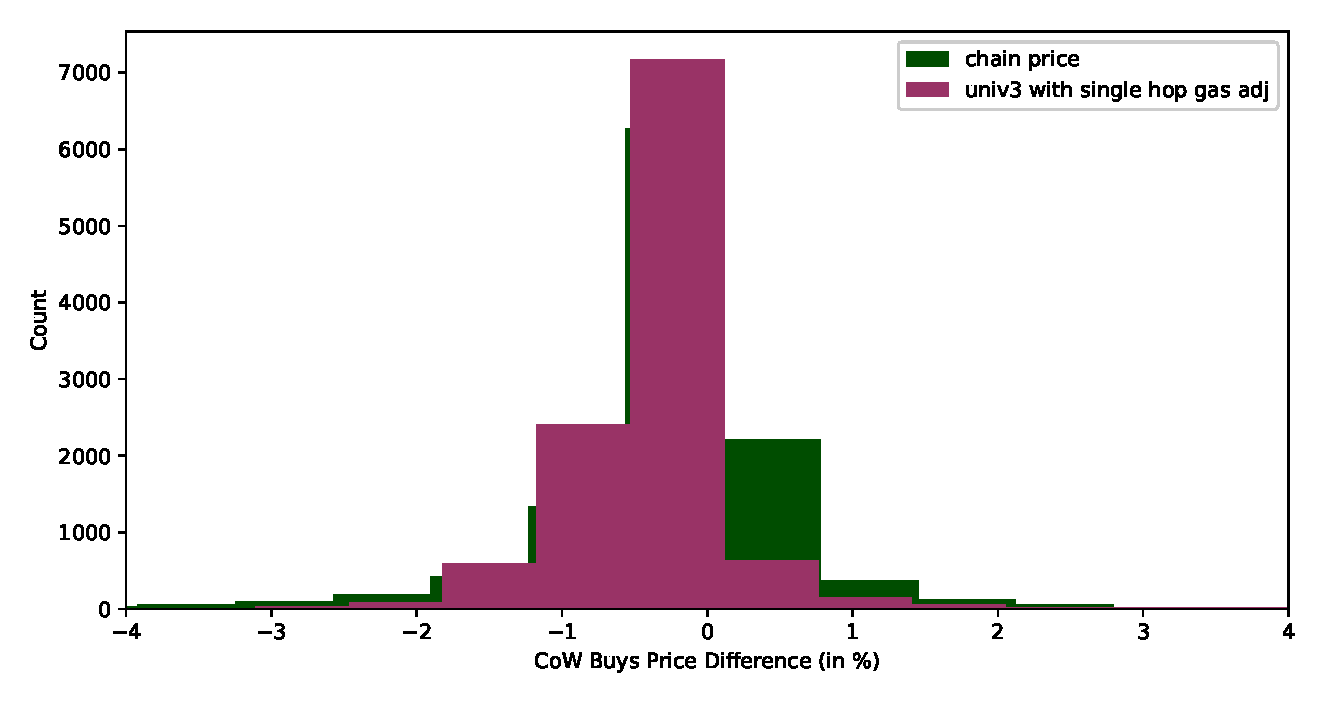
\includegraphics[width=.9\textwidth]
          {diagrams/weth_buy_hist.eps}
          %\caption{CoW price deviation, buying WETH for USDC}
      \end{center}
   \end{minipage}%
    %
    \begin{minipage}{.5\textwidth}
      \begin{center}
        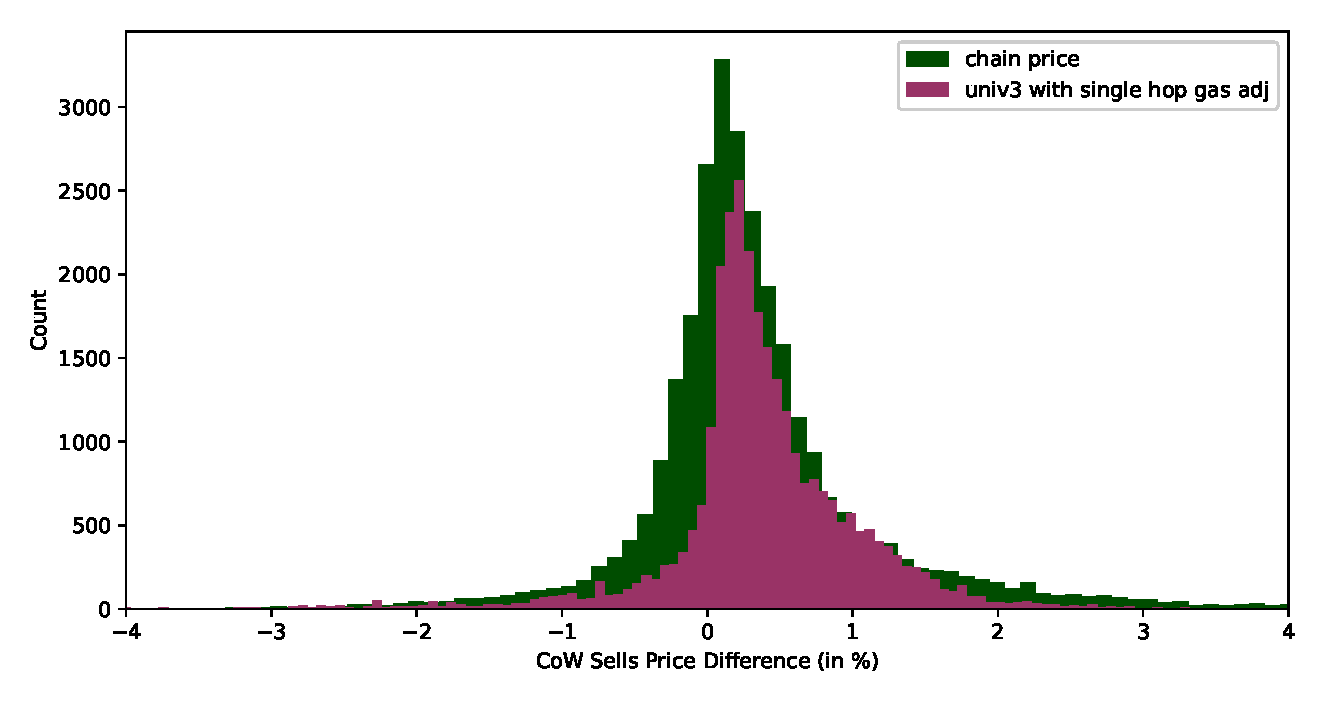
\includegraphics[width=.9\textwidth]
          {diagrams/weth_sell_hist.eps}
          %\caption{CoW price deviation, selling WETH for USDC}
      \end{center}
    \end{minipage}
  \end{center}
  \caption{WETH/USDC single hop gas adjustment price deviation on CoW, aggregated from August 2021 to March 2023 and separated into buy and sell side for CoW and Univ3. Note that sell count was 8,120 and the buy count was 3,025. The imbalance is attributed to the general market conditions during this period.}
\end{figure}

\begin{figure}
  \begin{center} 
    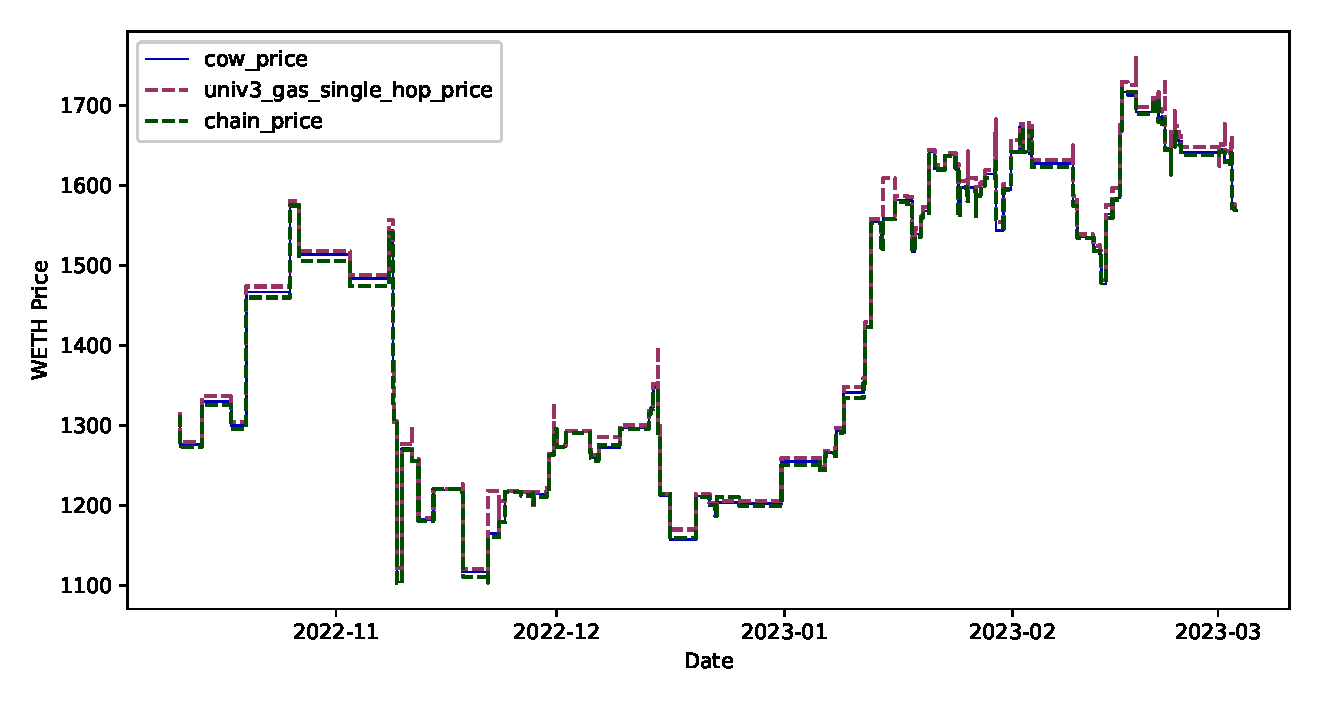
\includegraphics[width=\textwidth * \real{0.7}]{diagrams/weth_buy_line.eps}
    \caption{CoW buy side price execution compared to Uniswap v3 and Chainlink from October 2022 - March 2023}
  \end{center}
\end{figure}

\begin{figure}
  \begin{center} 
    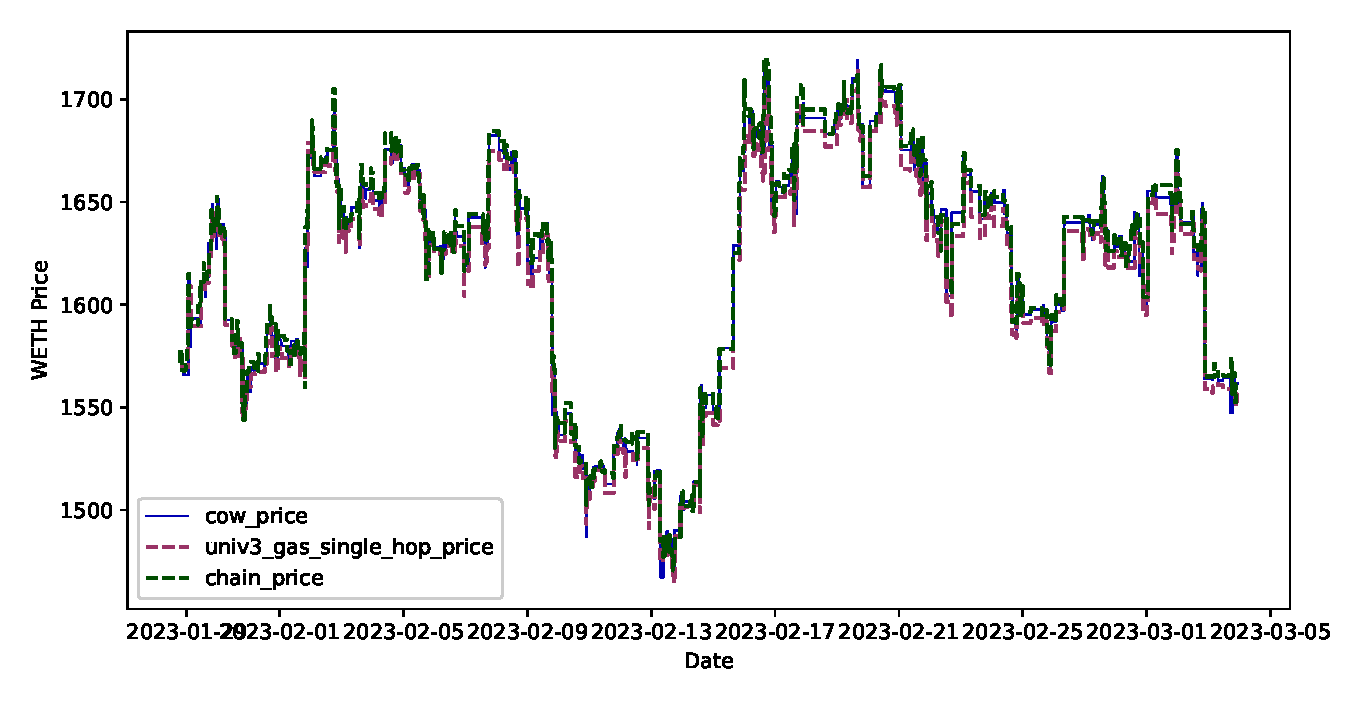
\includegraphics[width=\textwidth * \real{0.7}]{diagrams/weth_sell_line.eps}
    \caption{CoW sell side price execution compared to Uniswap v3 and Chainlink from October 2022 - March 2023}
  \end{center}
\end{figure}





\paragraph{Dataset.} Our dataset consists of Ethereum log data, which records certain on-chain events such as trades. It was sourced from The Graph, a blockchain data indexing service.\footnote{https://thegraph.com/}
%
More precisely, we used the Univ3, CoW, and Chainlink subgraphs curated by Messari, an analytics provider.\footnote{https://subgraphs.messari.io/}
%
Full details and our codebase are available [LINK TO FEEDLOT REPO?].

\begin{comment}
%To perform this task, we utilized the DataStreams python library, which is a subgraph query utility package. 
%We performed merges and data transformations with Polars.\footnote{link to Polar https://github.com/pola-rs/polars}
%Polars follows the Apache Arrow standards which is a in-memory columnar analytics standard in the industry. 
\end{comment}


\section{Conclusion}

A safe implementation of a Feedlot AMM on the subscription model would provide traders with cheap trading at up-to-date instantaneous market prices.
%
Unlike traditional static CFMMs, Feedlot protects LPs from adverse selection, while still offering an option to enjoy flexibly priced portfolio management. 
%
It would also yield a new revenue stream for CoW protocol in the form of oracle fees.

The question of whether a safe implementation is possible requires further research.
%
While the guarantees of CoW itself provide that a Feedlot oracle is always `truthful,' the difficult problem of preventing or discouraging the reporting of an `artificial' (albeit truthful) price --- a price under a centralised influence by a manipulatin attacker --- remains a challenge. 
%
A team wishing to implement a Feedlot AMM must take great care to ensure that it does not make the CoW UCP an economically viable target for manipulation, inviting harm on Feedlot LPs and users and stakeholders of CoW protocol alike.
%
Simply put, no one would want to provide liquidity to a pool which is forced to accept trades at any price quoted to it.

In \S\ref{manipulation}, we have established that some kind of volume controls are a necessary condition for manipulation resistance.
%
However, na\"ively limiting volume in terms of the volume on CoW is not sufficient, since this quantity is itself prone to relatively low-cost manipulation.
%
Furthermore, if the scale of traditional derivative markets is anything to go by, there is likely to be interest in increasing the allowable volume to many times the volume of the CoW batch itself.
%
We recommend that further resources be committed to research mitigation and enforcement methodology, with some more specific suggestions outlined in \S\ref{mitigation}.


\printbibliography
\end{document}
